\documentclass[oneside,final,14pt,a4paper]{extreport}

% \usepackage[T2A]{fontenc}
\usepackage[T1]{fontenc}
\usepackage{textcomp}

\usepackage{fontspec}
\setmainfont{Times New Roman}
\setmonofont{Courier}


\usepackage{vmargin}
\setpapersize{A4}
\setmarginsrb{2.5cm}{2cm}{2cm}{2cm}{0pt}{10mm}{0pt}{13mm}
\usepackage{setspace}
\sloppy
\setstretch{1.5}
\usepackage{indentfirst}
\parindent=1.25cm

%%%%% ADDED TO SUPPORT TT BOLD FACES %%%%
\DeclareFontShape{OT1}{cmtt}{bx}{n}{<5><6><7><8><9><10><10.95><12><14.4><17.28><20.74><24.88>cmttb10}{}
%%%%% END %%%%%%%%%%%%%%%%%%%%%%%%%%%%%%% 

\usepackage{atbegshi,picture}
\AtBeginShipout{\AtBeginShipoutUpperLeft{%
  \put(\dimexpr\paperwidth-1cm\relax,-1.5cm){\makebox[0pt][r]{
\includegraphics[width=3cm]{figs/inno}}}%
}}

% \usepackage[english]{babel}
\usepackage[russian]{babel}
\usepackage[backend=biber,style=ieee,autocite=inline]{biblatex}
\bibliography{ref.bib}
% \DefineBibliographyStrings{english}{%
%   bibliography = {References},}
\DefineBibliographyStrings{russian}{%
  bibliography = {Ссылки},}
\usepackage{blindtext}
\usepackage{pdfpages}
\newenvironment{bottompar}{\par\vspace*{\fill}}{\clearpage}
\usepackage{amsmath,amsfonts}

\usepackage{amsthm}
\newtheorem{theorem}{Theorem}
\newtheorem{corollary}{Corollary}
\newtheorem{lemma}{Lemma}
\newtheorem{proposition}{Proposition}
\theoremstyle{definition}
\newtheorem{definition}{Definition}
\theoremstyle{remark}
\newtheorem*{remark}{Remark}
\theoremstyle{remark}
\newtheorem*{example}{Example}

\usepackage{float}
\usepackage{graphicx}
\graphicspath{{figs/}} %path to images
\usepackage{array}
\usepackage{multirow,array}
\usepackage{caption}
\usepackage{subcaption}
\usepackage{hyperref}
\usepackage{paralist}

\usepackage{listings}
\lstset{basicstyle=\ttfamily,breaklines=true}

\usepackage{zed-csp}
\usepackage{fancyhdr}
\usepackage{csquotes}
\usepackage{color}

\usepackage{upgreek} 
\usepackage{bm}
\usepackage{hyperref}
\usepackage{setspace}
\usepackage{booktabs}
\usepackage{multirow}
\usepackage{longtable}
\usepackage[font=singlespacing, labelfont=bf]{caption}
\counterwithout{table}{chapter}
\renewcommand{\thetable}{\Roman{table}}
%Hints
\newcommand\pic[1]{(Fig. \ref{#1})} %Ref on figure
\newcommand\tab[1]{(Tab. \ref{#1})} %Ref on table


\usepackage{enumitem}
\newlist{inlinelist}{enumerate*}{1}
\setlist*[inlinelist,1]{%
  label=(\arabic*),
}

\usepackage[nopygments]{ffcode}




\pagestyle{fancyplain}

% remember section title
\renewcommand{\chaptermark}[1]%
	{\markboth{\chaptername~\thechapter~--~#1}{}}

% subsection number and title
\renewcommand{\sectionmark}[1]%
	{\markright{\thesection\ #1}}

\rhead[\fancyplain{}{\bf\leftmark}]%
      {\fancyplain{}{\bf\thepage}}
\lhead[\fancyplain{}{\bf\thepage}]%
      {\fancyplain{}{\bf\rightmark}}
\cfoot{} %bfseries


\newcommand{\dedication}[1]
   {\thispagestyle{empty}
     
   \begin{flushleft}\raggedleft #1\end{flushleft}
}

\begin{document}

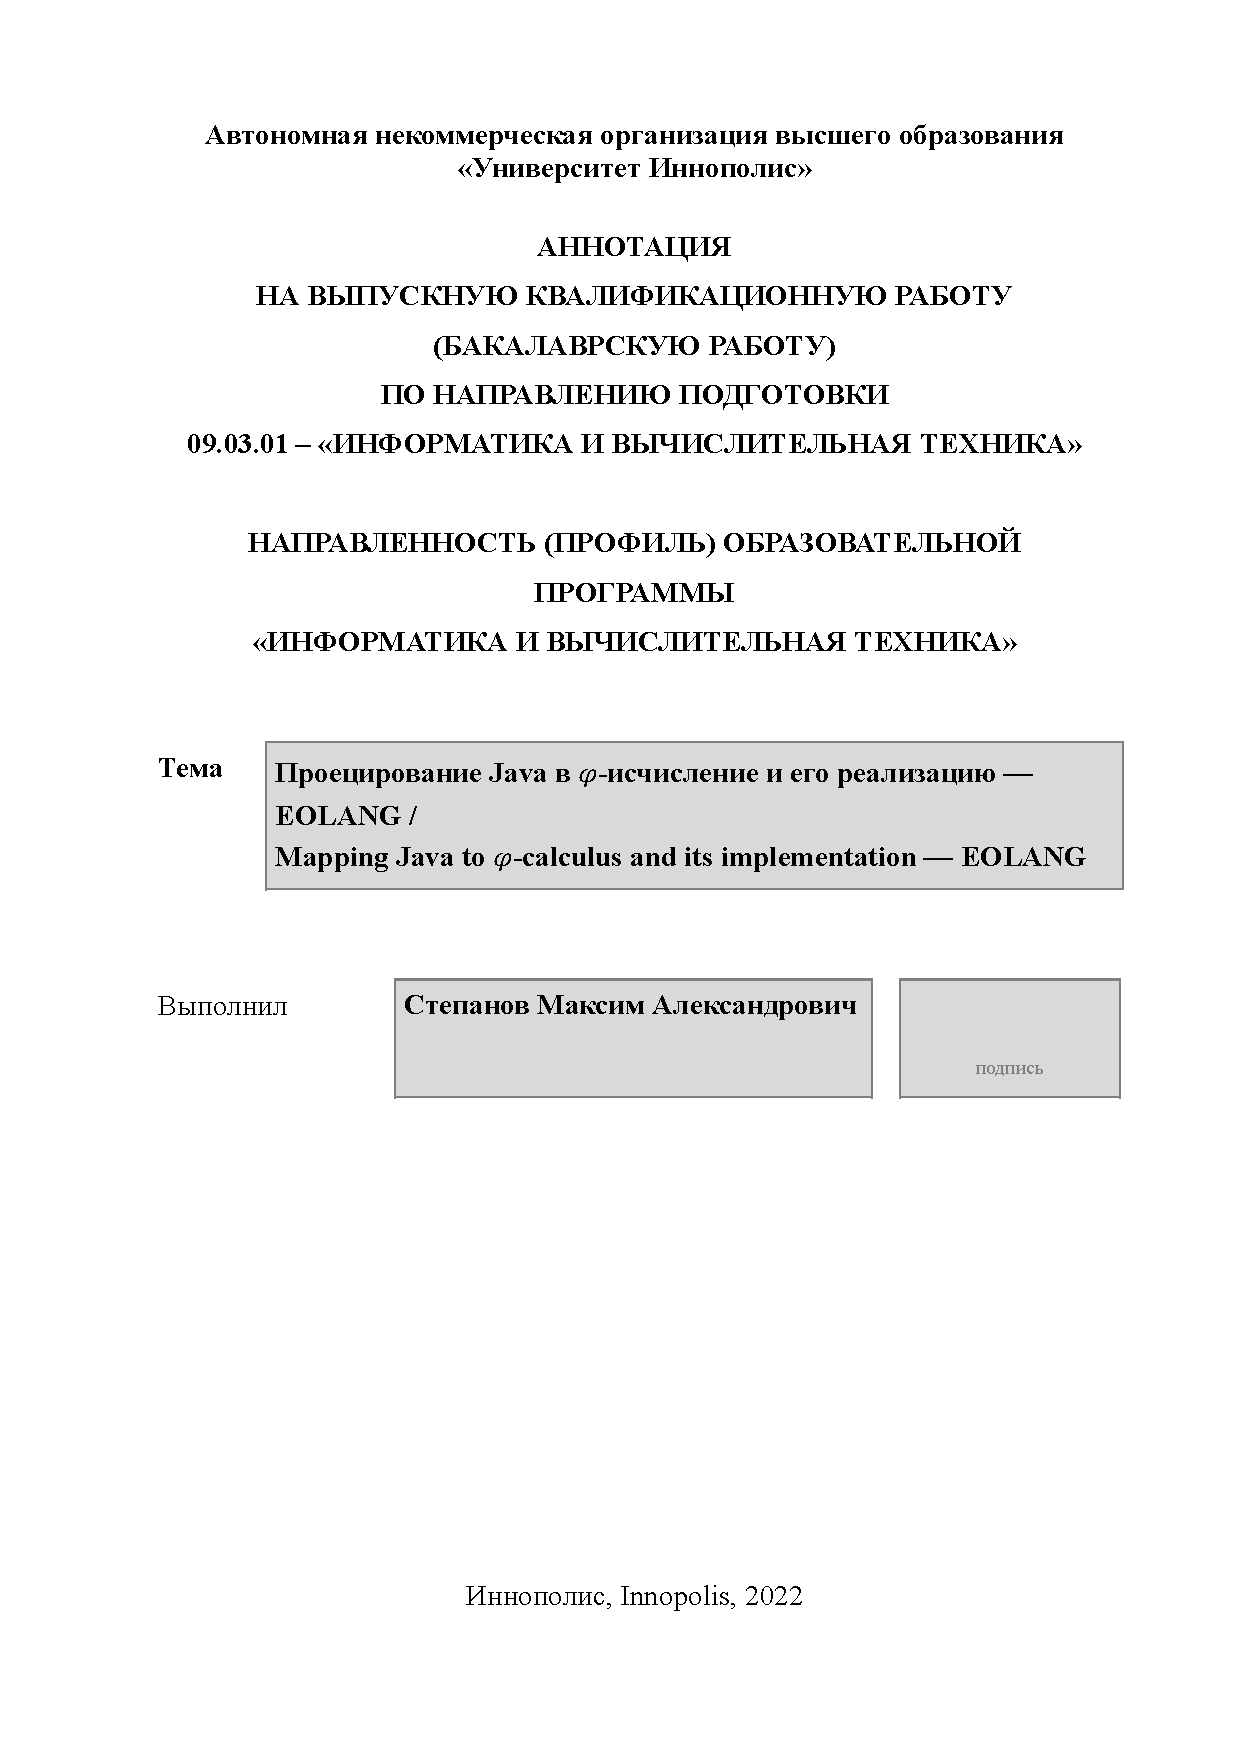
\includepdf[pages=-, offset=75 -75]{AnnotationTitle.pdf}
\tableofcontents
\listoftables
\listoffigures


\newpage

\begin{abstract}
  Данный диплом описывает способ проецирования традиционного объектно-ориентированного языка программирования (в частности --- Java) в $\varphi$-исчисление (конкретнее --- в его реализацию --- EOLANG). EOLANG накладывает определенные дополнительные ограничения поверх $\varphi$-исчисления, следовательно, транслятор, который разрабатывается как часть этого диплома, делает больший упор на реализацию проекта, чем на теорию проецирования.
\end{abstract}

% Depend on above part
\setcounter{page}{5}


\chapter{Введение}

Этот проект направлен на предоставление инструмента транспиляции исходного кода Java (\emph{исходный язык}) в EOLANG (\emph{целевой язык}) для передачи результата в статический анализатор Polystat \cite{polystat_repo} и его дальнейшего анализа.

Транспилятор (англ. transpiler), также часто называемый транслятором (англ. translator), представляет собой программный инструмент, который преобразует исходный код одного языка в исходный код другого языка. Транспиляция (англ. transpilation) или трансляция (англ. translation) --- это операция преобразования исходного кода с помощью такого инструмента.

EOLANG \cite{eolang_repo} — универсальное промежуточное представление семантики объектно-ориентированного языка, активно разрабатываемое в рамках проекта Polystat. Академическое сообщество еще не полностью изучило EOLANG и его формальную основу --- $\varphi$-исчисление, что придает диссертации \textbf{новизну} и является основной причиной его выбора в качестве целевого языка для проекта.

Согласно индексу TIOBE \cite{tiobe_index}, Java является третьим по популярности языком программирования. Индекс TIOBE — авторитетный показатель в области разработки программного обеспечения. Популярность языка придает \textbf{актуальность} проекту, что является основной причиной его выбора в качестве исходного языка для проекта.

Статический семантический анализ \cite{bardas2010static,epure2016semantic} является одним из популярных подходов к минимизации количества ошибок в программном проекте, и область статического анализа активно исследуется в настоящее время.

Общая цель Polystat — предоставить инструменты для перевода различных языков программирования в EOLANG и инструмент для выполнения обобщенного статического анализа промежуточного представления EOLANG. Такой подход позволяет реализовать единый универсальный инструмент анализа, охватывающий несколько объектно-ориентированных языков, сводя к минимуму усилия команды разработчиков анализатора Polystat, реализуя алгоритм анализа только один раз. Этот проект, J2EO, относится к первому типу инструментов — переводу Java в EOLANG. Структура всего проекта показана в \pic{fig:polystat_structure}.

\begin{figure}[H]
    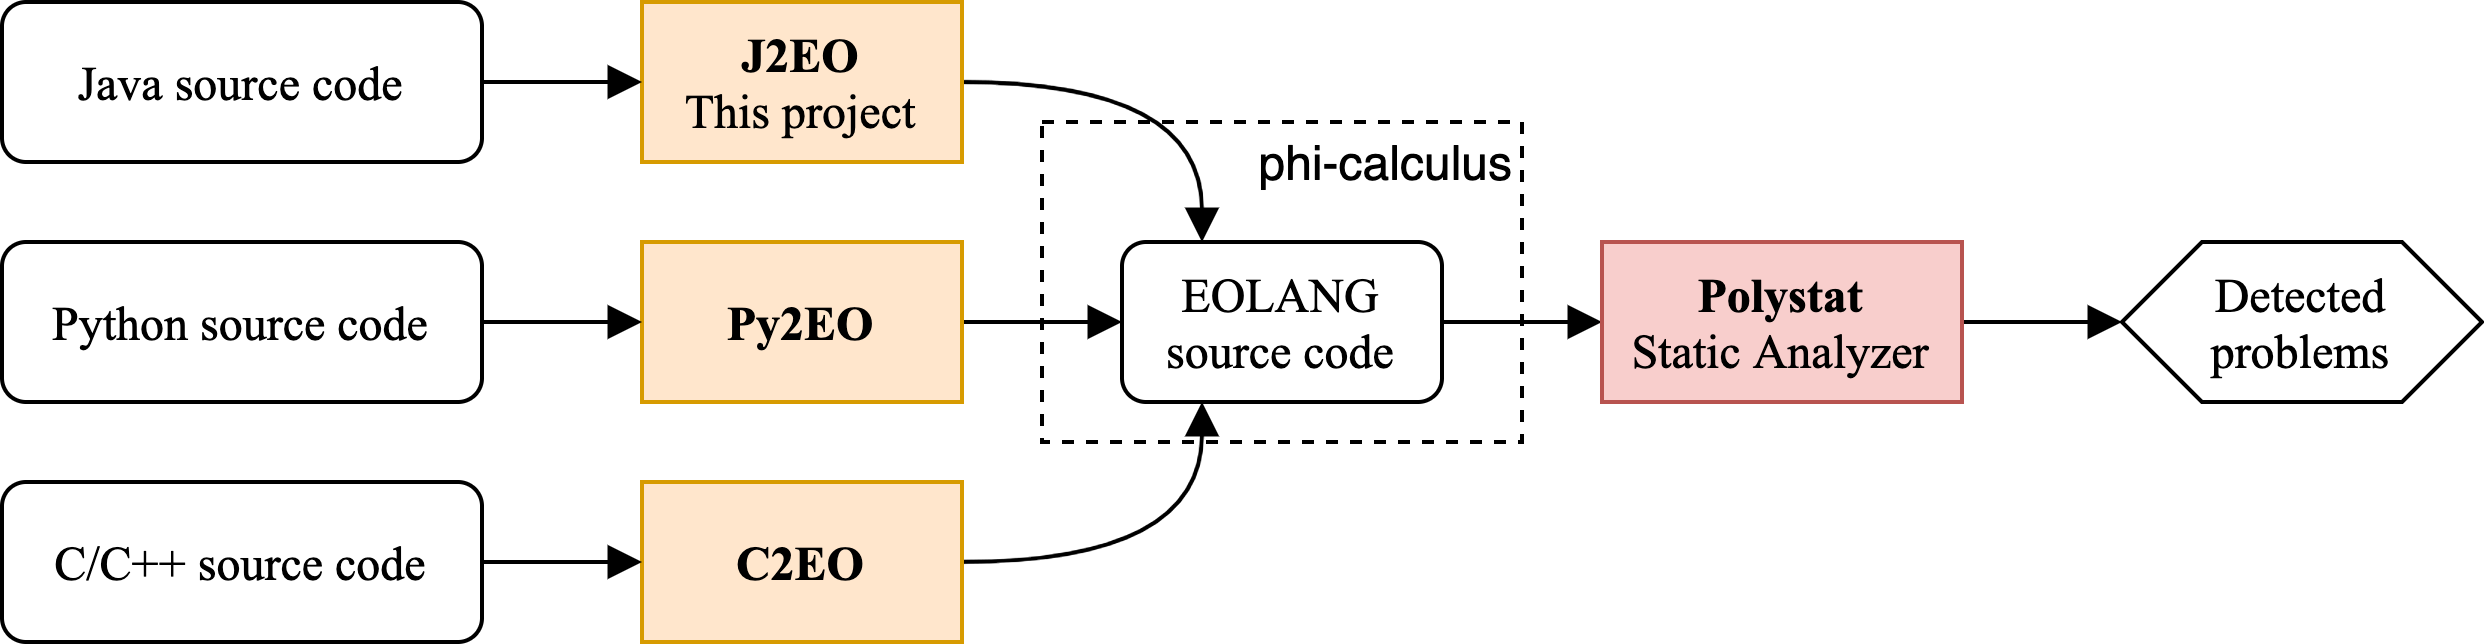
\includegraphics[width=1\textwidth]{polystat_structure.png}
    \centering
    \caption{Общая структура проекта Polystat}
    \label{fig:polystat_structure}
\end{figure}


\section{Обзор содержания тезиса}

В главе «Обзор литературы» будет изложена общая информация о трансляторах языков программирования, работе, проделанной в этой области, целях таких проектов, часто встречающихся проблемах и их решениях. Он также охватывает некоторые функции EOLANG и связанные с ними проблемы.

В главе «Реализация» будет подробно представлена ​​методология проектирования, а также описаны детали реализации проекта.

В главе «Результаты и обсуждение» будут представлены результаты реализованного проекта и обсуждены будущие возможности и актуальность проекта.


\chapter{Реализация}
\label{chapter:implementation}

В этой главе рассматриваются теоретические аспекты, связанные с переводом Java на EO, разработанные прогнозы и описание программного проекта, разработанного вместе с этим тезисом.


\section{Концептуальное сравнение Java и EO}
\label{section:conceptual_comparison}

Чтобы приступить к переводу одного языка на другой, важно понимать их отличия. Даже один и тот же термин может по-разному интерпретироваться разработчиками нескольких языков.

\subsection{Парадигма}

Важно помнить, что в прошлом различные языки, включая Java, искажали исходное представление об объектно-ориентированной парадигме. Таким образом, объектно-ориентированная парадигма по-разному интерпретируется разработчиками разных языков.

Java реализует традиционную в настоящее время парадигму ООП. Он строго вынуждает разработчиков помещать все в классы или интерфейсы, которые являются единственными доступными конструкциями верхнего уровня.

ЕО ближе к функциональной парадигме с упором на объекты. Он также претендует на то, чтобы быть языком ООП, хотя EO подразумевает исходное значение этого термина.

\subsection{Видимость}
Java имеет строгую систему видимости, включающую четыре уровня, описанные в
подразделе \ref{subsection:java_visibility}. ЕО, с другой стороны, не имеет
система видимости вообще. Такая система видимости невозможна в ЕО из-за его динамической природы, включая динамическую типизацию, отсутствие спецификации структуры объектов и неограниченный доступ к созданию и модификации объектов.
Эти функции необходимы для того, чтобы структура языка оставалась достаточно гибкой для перевода на нее различных языков.


\subsection{Изменчивость}
В Java все переменные по умолчанию изменяемы (англ. mutable) (хотя это может быть ограничено с помощью final). В EO нет встроенной поддержки изменяемости (англ. immutable), но есть обходные пути в стандартной библиотеке: \ff{memory} и \ff{cage}.


\subsection{Стиль программирования}
В языке Java используется императивный стиль: разработчик пишет код, который говорит \emph{как} выполнить программу. Декларативный стиль может быть достигнут с помощью специально реализованной пары исполнителя и структуры данных, но он не будет работать с библиотеками (как стандартной библиотекой, так и внешними библиотеками). Для поддержки библиотек необходимы пользовательские обертки.

EO имеет декларативный стиль --- разработчик пишет \emph{чего он хочет добиться}, а не как этого добиться. Императивный стиль может быть достигнут с помощью встроенного атома с именем \ff{seq}, но из-за особенностей реализации область \ff{seq} более ограничена, чем область действия объекта, например, невозможно объявить переменные внутри.


\section{Проекции}

В этом разделе будут рассмотрены теоретические подходы к проектированию исходного кода Java в семантически эквивалентный исходный код EO.

\subsection{Именование}
Java и EO имеют разные соглашения по именованию языковых компонентов, и если Java не обязывает использовать соглашения об именовании, EO это делает. Следовательно, отображение имен должно быть разработано и согласовано во всех трансляторах, чтобы результирующий код работал.

В частности: имена объектов и атрибутов в EO могут начинаться только с букв нижнего регистра и продолжаться буквами верхнего/нижнего регистра, цифрами, дефисами или символами подчеркивания. Это отличается от Java только первым символом, поэтому решение состоит в том, чтобы добавлять перед именами фиксированную текстовую последовательность.

Кроме того, у EO есть проблемы с затенением атрибутов. Затенение атрибутов — это функция языка, которая позволяет переопределять переменные (атрибуты в терминах EO) во вложенных областях. Эта функция работает непредсказуемым образом, особенно учитывая нестабильную природу EO (она все еще находится на ранней стадии разработки, и поведение часто меняется на момент написания этой статьи). Поэтому транслятор максимально избегает дублирования имен. Первым шагом к минимизации таких дубликатов является добавление разных типов токенов исходного кода с разными префиксами.

В качестве решения проблемы затенения атрибутов были разработаны следующие сопоставления:
\begin{itemize}
  \item Имена классов начинаются с \texttt{class\_\_}
  \item Переменные начинаются с \texttt{var\_\_}
  \item Аргументы начинаются с \texttt{arg\_\_}
  \item Методы начинаются с \texttt{method\_\_}
\end{itemize}


\subsection{Конструкторы}
Java, как и многие современные языки ООП, имеет конструкторы классов. В EO нет классов, поэтому реализация конструкторов находится под полным контролем транслятора. В текущей форме конструкторы Java отображаются в атрибуты функций с дополнительным именем \texttt{cons}.


\subsection{Перегрузка}
Кроме того, EO не поддерживает перегрузку методов/конструкторов и даже не имеет функций напрямую. Это простые объекты, как и все в языке. Поэтому к именам методов/конструкторов добавляются имена типов, разделенные \texttt{\_\_}. Информация о дженериках опущена, как это делает и JVM.

Пример результирующего сопоставления с учетом всего вышеперечисленного:
\begin{ffcode}
class A {
  A(int member) {...}
  void functionName(int arg1, Option<Value> arg2) {...}
}
\end{ffcode}

\begin{ffcode}
[] > class__A
  [] > new
    [] > this
      [var__member] > cons__int
        ...

      [] > method__functionName__int__Option
        ...
\end{ffcode}

\subsection{Выражения}
Java предоставляет способ создания сложных вложенных и связанных (разделенных точкой) выражений. Эти выражения могут вызывать различные побочные эффекты в разном порядке.


\subsubsection{Связанные выражения}

Сложный случай — цепные выражения. Из-за особого подхода к вызову функций в EO вызов метода экземпляра класса требует передачи этого экземпляра в качестве первого аргумента, то есть \texttt{obj.function(obj)}. Это легко сделать, когда используются операторы с одним выражением, но цепочка с точкой требует где-то хранить промежуточный объект, чтобы можно было продолжить цепочку.

Рассмотрим следующий пример на Java:

\begin{ffcode}
var result = obj.setValue(value).computeResult();
\end{ffcode}

\begin{ffcode}
... > obj
... > value
...
[obj] > <uuid_1>
  seq > @
    obj.setValue obj value
[obj] > <uuid_2>
  seq > @
    obj.computeResult obj
...
seq > @
  ...
  <uuid_2>
    <uuid_1>
      obj
\end{ffcode}

Хотя вариант EO требует значительно больше кода для выполнения той же операции, язык никогда не предназначался для написания кода вручную, а только для перевода с других языков.


\subsubsection{Побочные эффекты в выражениях}

Рассмотрим следующий фрагмент Java:

\begin{ffcode}
var out = obj.setValue(obj2.setValue(obj2.getCount()).i++);
\end{ffcode}

Он отличается от предыдущего фрагмента одной особенностью — операцией постинкремента, которая является побочным эффектом мутации на месте.

В этом коде в заданном порядке выполняются следующие операции:
\begin{itemize}
    \item Вызывается функция \texttt{getCount} из \texttt{obj2} и получается результат
    \item Функция \texttt{setValue} объекта \texttt{obj2} вызывается с полученным значением
    \item \texttt{obj2} возвращает себя для дальнейшего связанного вызова
    \item Получено свойство \texttt{i} объекта \texttt{obj2}
    \item Свойство \texttt{i} у \texttt{obj2} увеличивается на 1
    \item Функция \texttt{setValue} из \texttt{obj} вызывается со значением, полученным до увеличения, так как это тип значения, а не ссылочный тип
    \item Результат \texttt{setValue} присваивается \texttt{out}
\end{itemize}

Как видно из списка выше, порядок выполнения не соответствует абстрактному синтаксическому дереву, в частности --- операция постинкремента. Эту операцию нужно было ставить перед получением результата, как в преинкременте, чтобы соответствовать структуре AST. Этот факт измененного порядка затрудняет перевод Java-кода в EO, который не имеет соответствующего синтаксического сахара, а также переменных с типизированным значением.

Общая проблема заключается в том, что выражение вызывает побочные эффекты: EO не поощряет любые операции с побочными эффектами и предоставляет только «серые» обходные атомы для имитации побочных эффектов, для создания уровня совместимости с программами, основанными на побочных эффектах. Но поскольку типов-значений по-прежнему нет, нам приходится обходить операции, которые полагаются на них, с помощью специальной логики (т. е. создавать новую переменную).

Учитывая методы, описанные выше, мы можем получить следующее отображение ЕО:

\begin{ffcode}
... > obj
... > obj2
...
[obj] > <uuid_1>
  memory > result
  seq > @
    result.write
      obj.getCount obj
    result
[obj arg] > <uuid_2>
  seq > @
    obj.setValue obj arg
[obj] > <uuid_3>
  memory > result
  seq > @
    result.write
      obj.i
    obj.i.write
      add
        obj.i
        1
    result
[obj arg] > <uuid_4>
  seq > @
    obj.setValue
      obj
      arg
...
seq > @
  ...
  <uuid_4>
    obj
    <uuid_3>
      <uuid_2>
        obj2
        <uuid_1>
          obj2
  ...
\end{ffcode}


Обратите внимание, как реализован постинкремент в \texttt{<uuid\_3>}: создается новый объект \texttt{memory} (представьте его как ячейку, которая может хранить какое-то значение), туда копируется текущее значение, а затем значение исходного объекта обновляется.

Тот же подход используется везде, где используются типы значений (для Java список включает \texttt{int}, \texttt{long}, \texttt{short}, \texttt{char}, \texttt{float}, \texttt{double}). В данном случае он используется в \texttt{<uuid\_1>}. Это обеспечивает надежный способ гарантировать, что исходное значение не будет изменено последующими вызовами функций, поскольку оно не изменяется в Java.

\subsection{Разрешение составных имен в Java}
В Java есть очень неприятная особенность со ссылками на вложенные классы/члены: каждый токен в любом случае отделяется точкой. Поэтому невозможно сказать, какая именно операция представлена ​​конкретной точкой: является ли она частью имени пакета, ссылкой на класс из пакета или ссылкой на член класса.

Для определения работы составного имени анализируется блок импорта:
если строка из блока импорта Java (исключая последнюю часть, либо \texttt{*}, либо имя класса) является началом составного имени, части пакета не изменяются в составном имени EO; файл, на который ссылается имя пакета, загружается, анализируется и анализируется. Части, которые соответствуют именам классов, начинаются с \texttt{class\_\_}, части, которые соответствуют именам переменных, начинаются с \texttt{var\_\_}.


\subsection{Отображение классов}
% <вставить ссылку на документ конференции>
% <копия из статьи J2EO>

Тела классов достаточно просто перевести.
\begin{itemize}
  \item Класс – это объект со всеми статическими членами и статическими методами, а также фабрикой объектов \texttt{new} и конструкторами \texttt{cons<n>}. Он также украшает суперкласс, наследуя его статические члены и методы.
  \item  Метод  \texttt{new} украшает объект суперкласса \texttt{new} и определяет члены класса с их значениями по умолчанию.
    \item \texttt{cons<n>}, содержащий соответствующий код конструктора Java.
\end{itemize}

Что представляет собой проблему, так это наследование, особенно множественное наследование (реализованное через интерфейсы в Java). Наблюдаемых подходов к интерфейсам карт в проекте пока нет, поэтому пока их пропустим. Основное внимание будет уделено урокам картирования.

Суперкласс записывается в атрибут \texttt{super} экземпляра при его создании.


Ниже приведен пример сопоставления классов:

Оригинальный фрагмент кода Java:

\begin{ffcode}
class A {
  int i = 42;
  int getI() { return i; }
}
class B extends A {
  int i = 1;
  B() { super(); i = 2; }
  int getI() { return i; }
  int getSuperI() { return super.i; }
  int setSuperI(int i) { super.i = i; }
}
\end{ffcode}

Производится семантически эквивалентный код ЕО:
\begin{ffcode}
[] > class__A
[] > new
  [] > this
    memory > i
    [this] > getI
      this.i > @
  seq > @
    this.i.write 42
    this
[this] > cons1
  this > @

[] > class__B
[] > new
  [] > this
    class__A.new > super
    super > @
    memory > i
    [this] > getI
      this.i > @
    [this] > getSuperI
      this.super.i > @
    [this i] > setSuperI
      seq > @
        this.super.i.write i
        this
  seq > @
    this.i.write 1
    this
[this] > cons1
  class__A.cons1 this > this2
  seq > @
    this2.i.write 2
    this2
\end{ffcode}

\subsection{Отображение интерфейсов}

Особенностью EO, которая позволяет расширять другие объекты, является декорация. Однако декорация позволяет моделировать только одиночное наследование. Java 8 привнесла в интерфейсы методы по умолчанию, что позволило реализовать множественное наследование. Это не вписывается в $\varphi$-исчисление, поэтому его можно только обойти, а не реализовать.

Текущее решение просто игнорирует интерфейсы, поскольку в основном они используются для облегчения статической проверки когда необходимо скрыть данные. Однако этот подход некорректно работает с методами по умолчанию.


\section{Обзор реализации J2EO}

В дополнение к теоретическим отображениям, продуктом диссертации является программный проект под названием J2EO. Проект написан на Java/Kotlin, а парсер использует ANTLR \cite{antlr_website}.

Обработка одного файла Java через разные модули показана ниже.

\begin{figure}[H]
  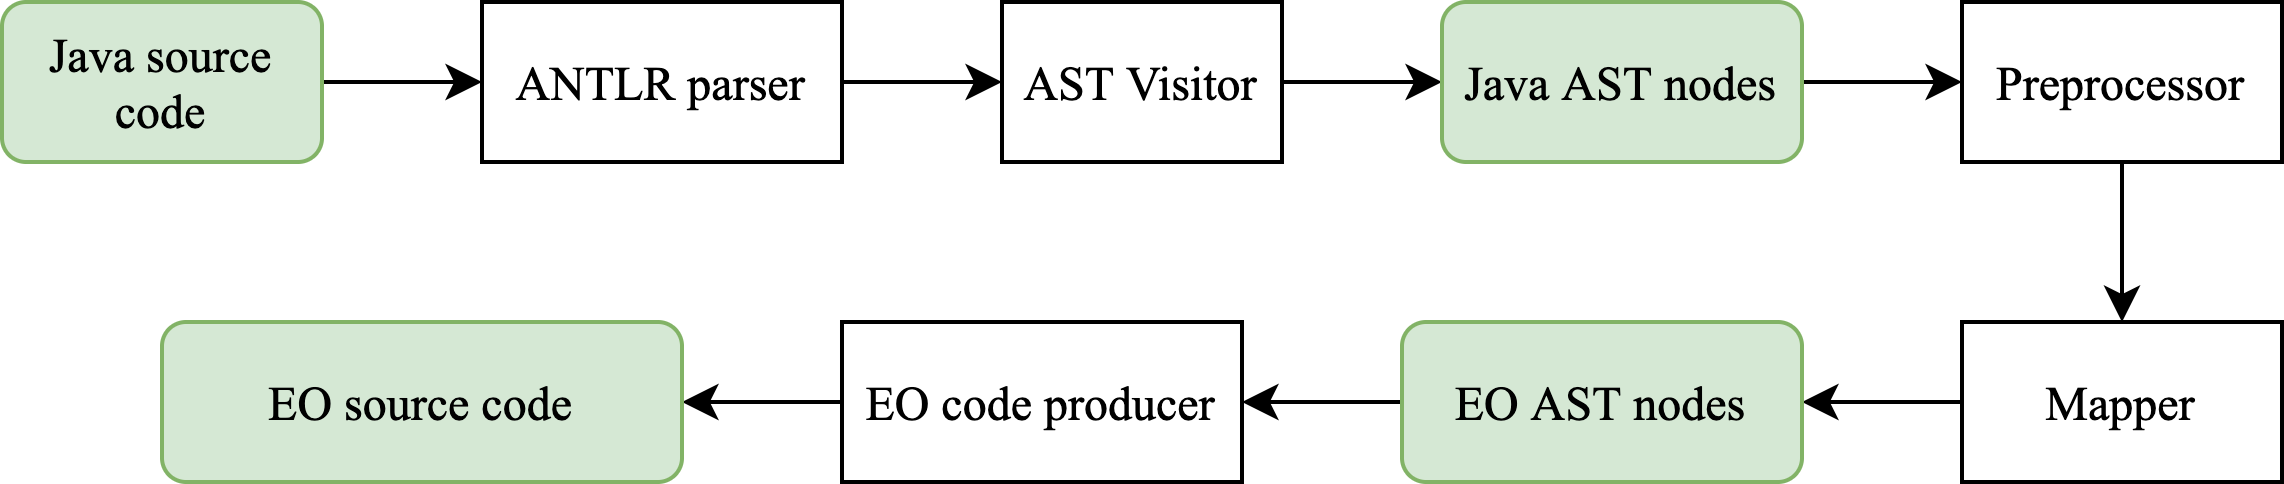
\includegraphics[width=1\textwidth]{j2eo_structure.png}
  \centering
  \caption{Обработка одного файла Java через конвейер J2EO}
  \label{fig:j2eo_flow}
\end{figure}

Обертка, которая обрабатывает ввод-вывод, выполнение конвейера и другие рутинные задачи, не рассматривается в этом тексте.

Следующая часть описывает каждый из шагов более подробно.

\subsection{Парсер ANTLR}
Парсеров Java для современных версий языка почти нет в Интернете. Единственный синтаксический анализатор, который охватывает Java 17, реализован в ANTLR и доступен на GitHub \cite{antlr_java_parser}. Требуются небольшие модификации, чтобы заставить его работать в случае использования J2EO.

\subsection{Посетитель AST}
Этот этап конвейера запускает синтаксический анализатор ANTLR и посещает каждый узел для создания внутреннего узла Java AST. Этот шаг необходим, поскольку ANTLR сам по себе не генерирует узлы AST, а только предоставляет контекст, который можно использовать для получения частей дерева.

\subsection{Препроцессор}

Препроцессор применяет исправления соглашения об именах к коду. Этот шаг включает префикс классов с \ff{class\_\_}, переименование импорта в соответствии с соглашениями EO и другие семантически-нейтральные изменения.

\subsection{Проектор}

Это основной шаг конвейера, который создает узлы EO AST из предварительно обработанных узлов Java AST. Методология проецирования узлов AST представлена в предыдущем разделе.

\subsection{Принтер кода EO}

Последним этапом конвейера является создание исходного кода из EO AST. Эта часть реализована в виде функций расширения Kotlin, которые добавляют методы к узлам EO AST неинвазивным способом.

\subsection{Подведение итогов}

Все описанные выше этапы пайплайна реализованы в функциональном стиле. Таким образом, ни одна из функций не использует общее изменяемое состояние, что позволяет распараллелить перевод файлов. Параллельная версия J2EO успешно протестирована.

Проект J2EO имеет открытый исходный код и доступен на GitHub. Любой может использовать его и внести свой вклад в него.




\chapter{Результаты и обсуждение}
\label{chapter:results_and_discussion}

\section{Результаты}

Результатом этой диссертации является часть программного обеспечения J2EO, написанного на Java/Kotlin. Реализованная часть включает в себя абстрактное синтаксическое дерево EO (AST), алгоритм, который печатает EO AST в файл с исходным кодом, и алгоритм, который переводит выбранные узлы Java AST в EO AST.

Основным вариантом использования J2EO является преобразование реальных проектов Java в EO для последующего выполнения статического анализа с другими проектами Polystat. Таким образом, важно без сбоев переводить большие проекты и максимизировать количество переведенных функций Java. Создание полного семантически эквивалентного кода не является обязательным требованием для статического анализа.

В качестве эталона для оценки результатов я выбрал несколько крупных проектов, активно используемых в промышленных системах.

Таблица использованных проектов с соответствующими им фактическими хэшами коммитов указана в таблице \ref{table:benchmark_projects}:

\begin{table}[H]
  \centering
  \begin{tabular}{| c | c | c | p{5cm} |} 
      \hline
      Project & Java version & LoC & Actual commit hash \\
      \hline
      Hadoop \cite{hadoop_repo} & 8 & 1631465 &   ec0ff1dc04b2ced199d7- 1543a8260e9225d9e014 \\
      \hline
      Kafka \cite{kafka_repo} & 8 & 499373 & f36de0744b915335de6b- 636e6bd6b5f1276f34f6 \\
      \hline
      J2EO \cite{j2eo_repo} & 17 & 41200 & a762a903eb55f3e11403-d4630654f4c89397d75a \\
      \hline
  \end{tabular}
  \caption{Java projects used for benchmarking}
  \label{table:benchmark_projects}
\end{table}

Используемая версия J2EO — 0.5.3, она присутствует в репозитории GitHub \cite{j2eo_repo} проекта.

Метрика Lines of Code (LoC) была рассчитана с помощью утилиты \ff{cloc}\cite{cloc} и включает только физические строки Java, исключая пустые строки и комментарии.

Данные версии программного обеспечения и хэши коммитов позволяют читателям воспроизводить результаты, приведенные в тексте, на своей машине.

\subsection{Расчетные проекции}

В рамках этой диссертации разработаны теоретические прогнозы для многих конструкций и функций Java. Полный список представлен в главе \ref{chapter:implementation}.

\subsection{Реализованные прогнозы}

На момент написания проекции, реализованные в J2EO, охватывают отображение классов, их статических и нестатических членов, статических и нестатических методов, поддержку большинства операторов, которые имеет смысл статически анализировать. Любая структура проекта анализируется правильно, поэтому в качестве входных данных могут быть переданы как проекты Maven, так и проекты Gradle с произвольной структурой каталогов.

Приоритет реализации проекций активно обсуждался с командой разработчиков анализатора, поэтому включенные отображения актуальны для дальнейшего развития всего суперпроекта.

Поддерживаемая версия Java — 17, и, учитывая обратную совместимость, поддерживаются любые проекты более ранних версий. Несколько записей в таблицах бенчмаркинга подтверждают это.

\subsection{Оценка результатов}

На момент написания статьи объективная оценка результатов невозможна, так как анализатор Polystat находится на ранних этапах разработки и, следовательно, не существует полного пайплайна анализа.
Основным используемым методом оценки является перевод больших проектов Java и проверка правильности созданных файлов EO вручную. Проекты из таблицы бенчмаркинга предоставляют кодовую базу из нескольких миллионов строк кода на Java и факт того, что транслятор успешно их обрабатывает звучит многообещающе для будущего этого проекта.


\section{Обсуждение и заключение}

В тексте представлен обзор используемых технологий, включая Java, EOLANG и $\varphi$-исчисление, затем дана оценка этих технологий для целей проекта, теоретические проекции конструкций между исходным и целевым языками и, наконец, описаны реализация самого инструмента.

Проект J2EO уже охватывает значительный диапазон функций Java, облегчая дальнейшую разработку анализатора Polystat. Поскольку Полистат сильно зависит от результатов работы транспиляторов, его разработка была приостановлена ​​на длительный период, и поэтому на момент написания статьи не было представлено никаких подробных результатов анализа.

Комбинация J2EO/Polystat все еще находится в активной разработке. Однако, по результатам J2EO, EO обеспечивает необходимую базу для представления других языков. Эта комбинация имеет все шансы стать конкурентоспособной с другими популярными статическими анализаторами Java, такими как PMD, SpotBugs и встроенным статическим анализатором IntelliJ IDEA (который недоступен отдельно).

Текущее исследование проекций Java в EOLANG и инструмент перевода J2EO будут представлены академическому сообществу в готовящейся к выпуску статье позже в этом году.


%% REFERENCES
\printbibliography[heading=bibintoc,title={Использованная библиография}]
\end{document}